\section{Ristrutturazione schema E-R}
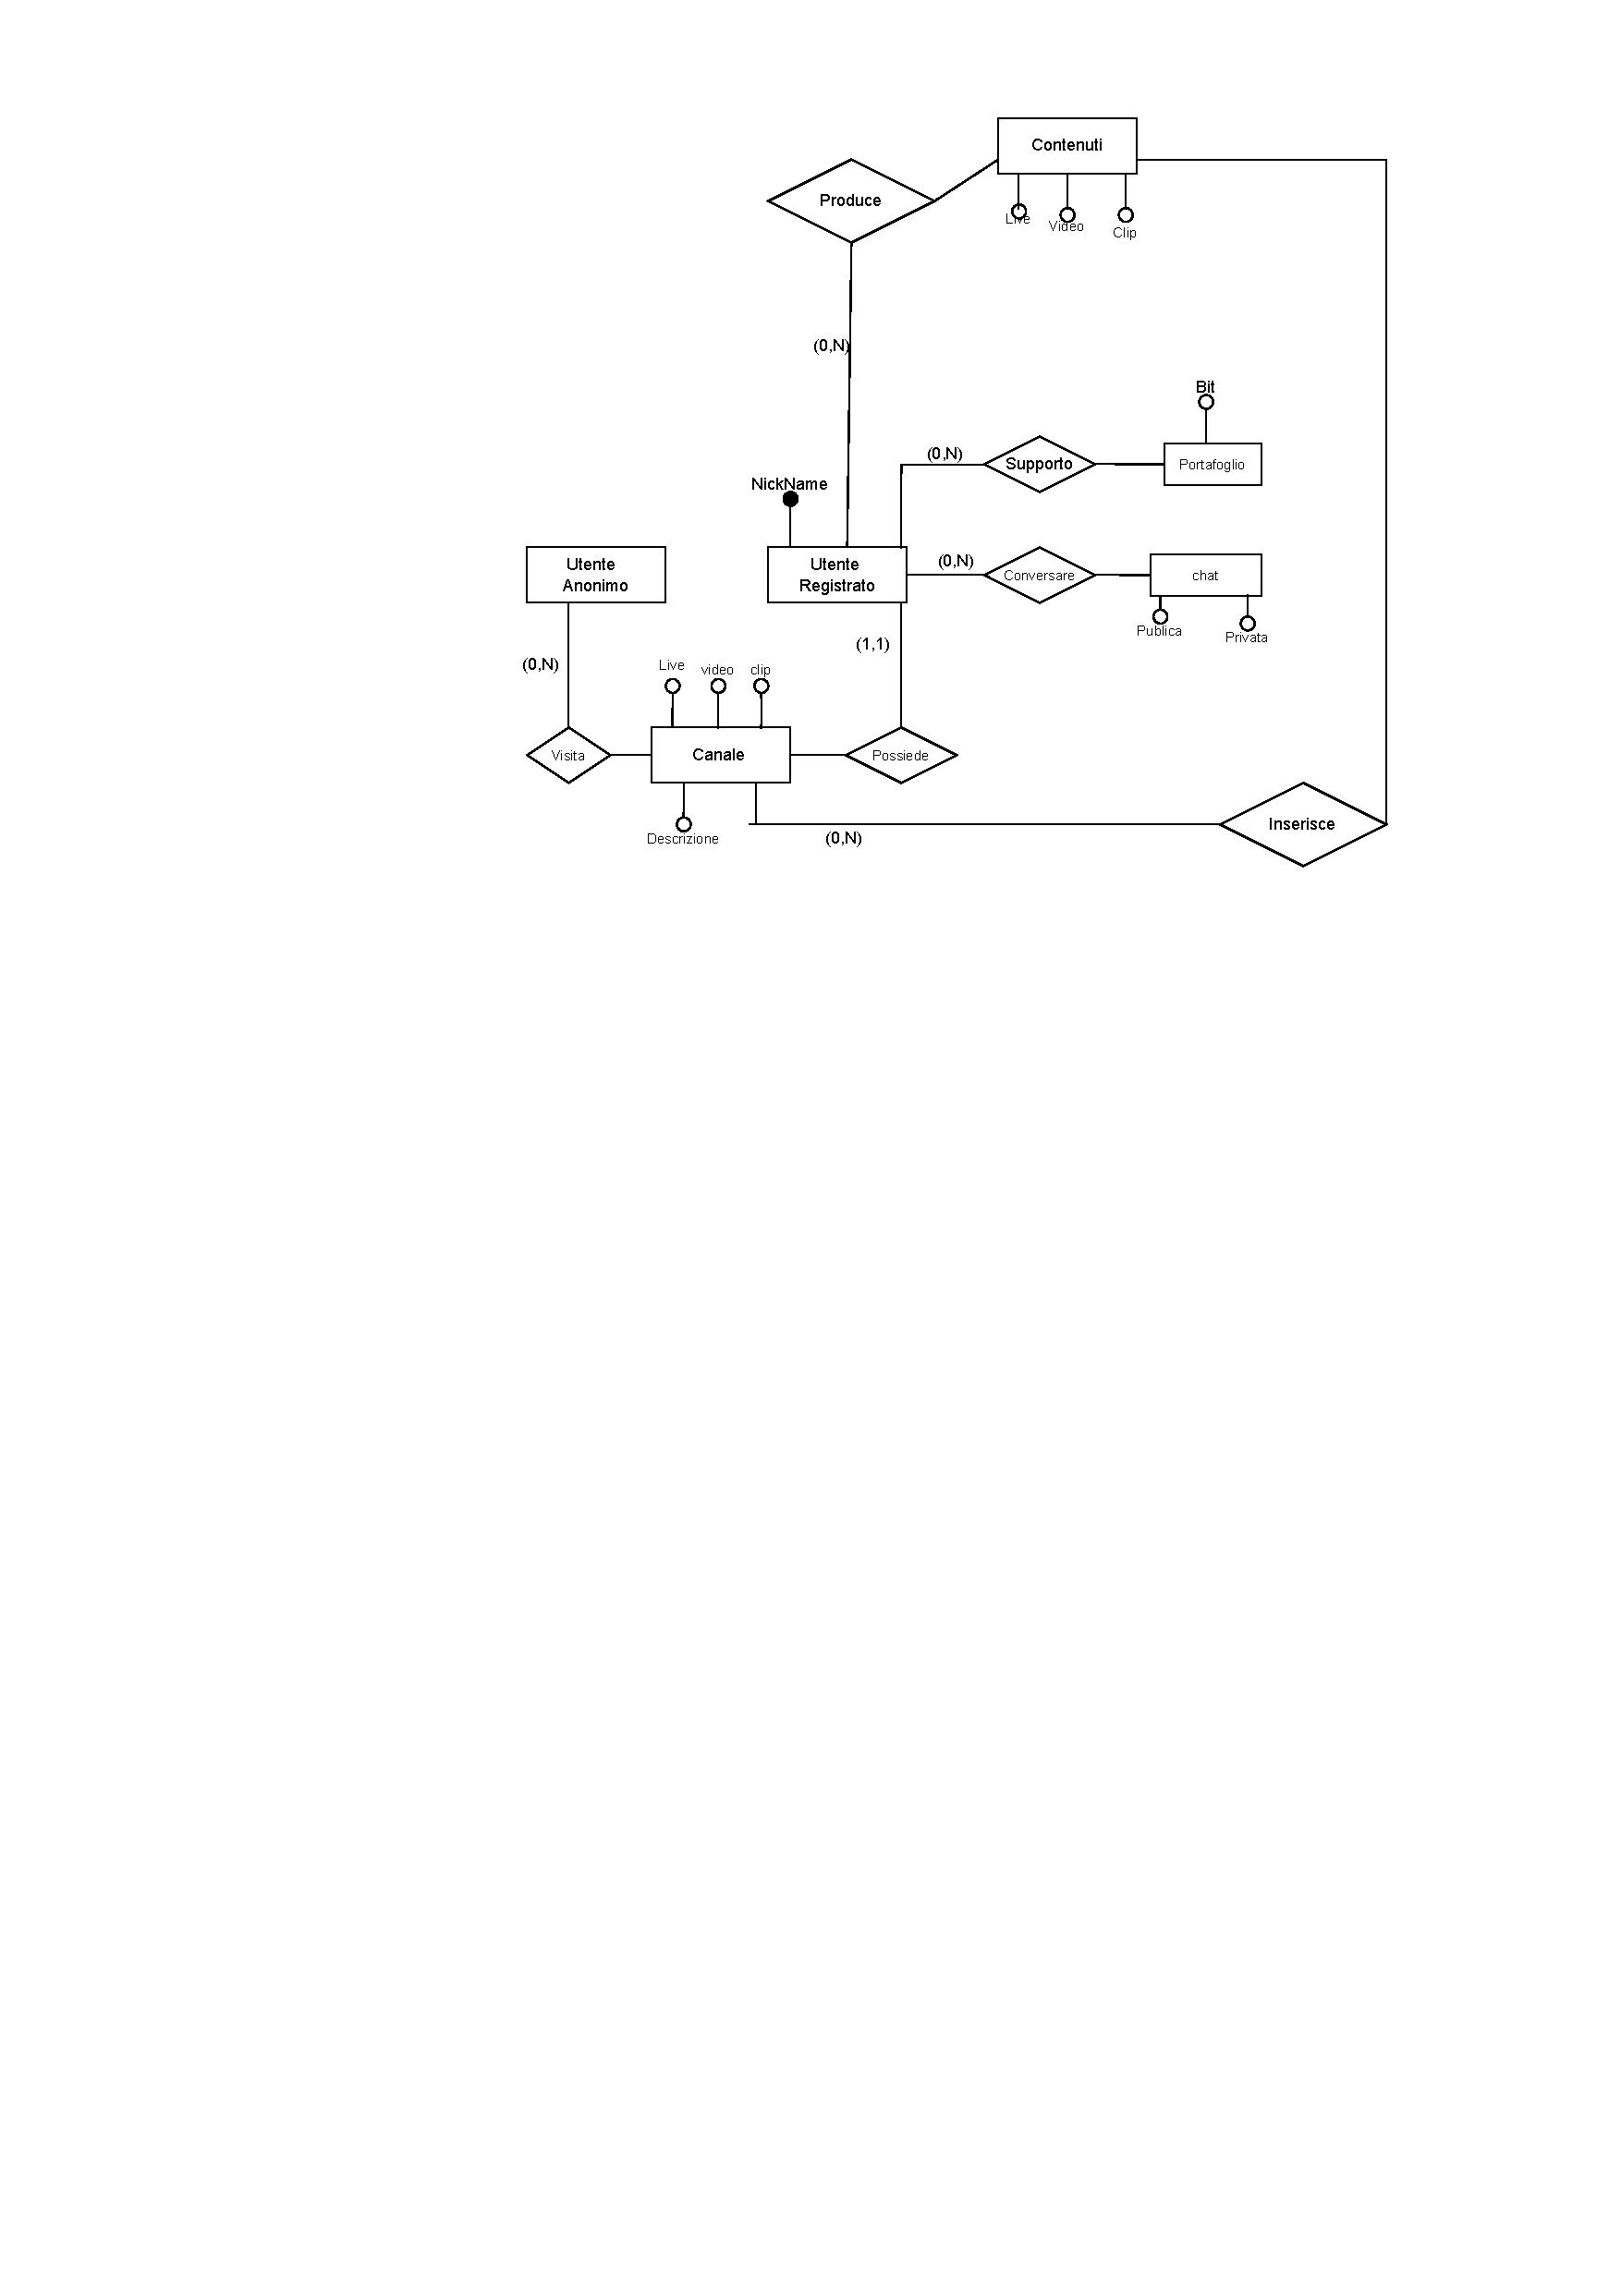
\includegraphics[width=\textwidth]{resources/e_r_ridotto.pdf}

\section{Analisi delle Generalizzazioni}
Le generalizzazioni presenti nello schema E-R sono:
\begin{enumerate}
    \item \textbf{Utente}: È una generalizzazione totale tra le entità \textit{Utente registrato} e \textit{Utente anonimo}, poichè o si è registrati alla piattaforma o si è anonimi
    \item \textbf{Streamer e Streamer-Spettatore}: È una generalizzazione parziale tra le entità \textit{Streamer} e \textit{Streamer-Spettatore}, in quanto l'utente registrato si ritrova a svolgere il ruolo o di streamer o di spettatore, ma sempre essendo uno streamer  
    \item \textbf{Spettatore - Utente Anonimo}: È una generalizzazione sovrapposta, poiché l'utente anonimo può essere solo spettatore'
    \item \textbf{Chat}: È una generalizzazione totale tra le entità \textit{Chat privata} e \textit{Chat pubblica}. Perché l'entià chat si divide in due sottoinsiemi, ovvero chat pubblica e chat privata.
\end{enumerate} 
\section{Partizionamento/Accorpamento di entità e associazioni}
Si è deciso di accorpare l'entità chat, così indica in maniera più coincisa che un utente registrato può comunicare in maniera pubblica o privata'''
\begin{figure}[ht]
    \centering
    \begin{minipage}{.45\textwidth}
        \centering
        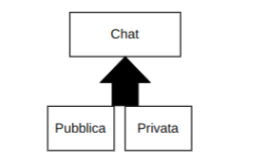
\includegraphics[width=0.9\linewidth]{resources/chat_revised.png}
        \caption{Entità chat dopo l'accorpamento}
        \label{fig:image1}
    \end{minipage}%
    \begin{minipage}{.5\textwidth}
        \centering
        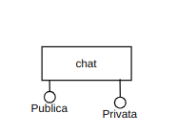
\includegraphics[width=0.9\linewidth]{resources/chat.png}
        \caption{Entità chat prima dell'accorpamento}
        \label{fig:image2}
    \end{minipage}
\end{figure}

\section{Business rules dell'E-R ristrutturato }
\begin{itemize}
    \item Gli attributi live ,video ,clip presenti nell'entità \textbf{canale} indicato un oggetto finito e caricato al suo interno.
    \item Gli attributi live ,vide ,clip presenti sull'entitá \textbf{contenuti} indicano un oggetto che ancora o è in fase di produzione o è un prodotto finito ma non caricato sul canale del proprietario. 
    \item Gli utenti anonimi non possono supportare gli streamer. 
    \item Gli streamer sono utenti registrati che caricano  o trasmettono contenuti. 
    \item Ogni utente registrato ha un nickname. 
    \item Il nickname scelto dall'utente registrato sarà anche il nome del canale. 
    \item Ogni canale ha una Descrizione. 
    \item Le live sono contenuti o in tempo reale.
    \item I video sono live già concluse. 
    \item Le clip sono brevi estratti di video. 
    \item Un utente anonimo non può conversare con altri utenti.
    \item Un utente anonimo non possiede un canale. 
\end{itemize}
